\chapter{Agenții algoritmici}
\section{Arhitectura clasei de bază}
\subsection{Interfața Player}
Integrarea cu sistemul de simulare a reprezentat o decizie importantă de proiectare a design-ului, dat fiind complexitatea deciziilor și multitudinea de cazuri ale apelării acestora. De aceea, am căutat o soluție cât mai eficientă și ușor de implementat, care să ofere o posibilitate simplă de scalare.

Astfel, un răspuns imediat a fost acela al folosirii unei clase de bază, care să expună metode corelate direct cu acțiunile întreprinse în cadrul jocului. Interfața Player rezolvă această problemă prin definirea acțiunilor necesare comunicării cu sistemul de simulare într-o manieră explicită, pe care mai apoi, fiecare agent le poate suprascrie în ideea optimizării lor și implementării unei politici particularizate.

\subsection{Metodele expuse}
Așa cum am arătat în tabelul \ref{fig:monopoly_actions}, acțiunile pentru interacționarea cu mediul au fost transpuse în metode ale clasei, corelate direct. Astfel regăsim printre acestea metodele prezentate în figura \ref{fig:player_interface_methods}.

\begin{figure}[h]
    \centering
    \includegraphics[width=16cm]{images/player_interface_table (1).png}
    \caption{Metodele Interfeței Player}
    \label{fig:player_interface_methods}
\end{figure}

\subsection{Sistemul de evenimente}
Prin intermediul EventManager \ref{event-manager}, orice acțiune întreprinsă de orice agent este considerată un eveniment în mediul implementat și partajată cu toți agenții participanți la joc, inclusiv cel care a efectuat acțiunea. Astfel, fiecare agent poate întreprinde o procesare suplimentară și actualiza baza proprie de cunoștințe cu scopul îmbunătățirii dinamice a politicii și adaptării la condițiile curente de joc.

Interfața player oferă o deja o implementare minimalistă a stocării evenimentelor și metode de ștergere și recepționare al unui eveniment pentru a ușura procesările ulterioare.

\section{Agentul aleator (random)}
Reprezintă agentul de bază (baseline) menit să fie un punct de referință în antrenare și stabilirea scopului. Acesta se bazează integral pe explorare și nu are niciun mecanism de îmbunătățire internă care ar fi favorizat exploatarea cunoștințelor dobândite, toate deciziile sale fiind aleator alese dintr-o distribuție probabilistică uniformă. Pentru îmbunătățirea vitezei și o procesare mai rapidă, o coadă de decizii binare este generată la inițializare și stocată, având o capacitate predefinită.

Beneficiile acestui agent sunt viteza de execuție și oferirea unei distribuții uniforme de acțiuni, astfel fiind un adversar impredictibil în fața căruia, strategiile fixe pot uneori eșua. Ca și dezavantaje, acesta nu va putea oferi strategii plauzibile sau reproductibile, fiind doar un punct de plecare în evaluarea agenților.

\section{Agentul algoritmic}
Agentul algoritmic este un punct de introducere în segmentarea și evaluarea deciziilor în jocul Monopoly. Așa cum am expus și mai sus, formalizarea unei strategii optime și găsirea unui algoritm general este un lucru greu de concretizat și poate crea mai multe ramificări în procesul decizional. De aceea, prin prezentul agent se încearcă o cuantificare superficială a modului de joc uman, care se bazează pe o analiză calitativă și cantitativă a planșei de joc și a tuturor elementelor implicate înainte de a acționa.

O distincție majoră față de agentul aleator o reprezintă evaluarea deciziei de cumpărare a unei proprietăți, aceasta făcându-se pe baza utilității sale în completarea de monopoluri, a favorizării aterizării pe proprietăți frecventate cu planificare pe termen lung, a observării probabilistice a profitului generat și nu în ultimul rând, analiza resurselor de care dispune, pentru evitarea aducerii într-o situație în care banii cash ar scădea sub un prag predeterminat.

De asemenea acesta analizează atent și deciziile precum îmbunătățirea proprietăților, ipotecarea acestora, folosirea cardurilor de ieșire din închisoare, etc. având în vedere mai mulți factori, precum fluiditatea cash-ului, completarea de monopoluri ale adversarului, riscul de faliment.

Algoritmul va încerca și tranzacționarea resurselor cu alți jucători, propunând și acceptând schimburi favorabile. Din păcate, această acțiune este una foarte greu de modelat practic, iar din experiențele observate, agentul tinde să tranzacționeze sume absurde pentru proprietăți care nu i-ar aduce niciun beneficiu vizibil.

Tratarea excepției de faliment se va face prioritizând păstrarea proprietăților de interes, în consolidarea monopolurilor, și se va încerca vânzarea celor care nu reprezentau un avantaj clar în câștigul jocului.

\section{Agentul strategic și variațiunile sale}
Agentul algoritmic reprezintă un punct definitoriu de plecare în problematica generalizării unei politici optime, dar acesta are dezavantajul gestionării slabe și a unei puteri slabe de procesare comparativ cu un inamic uman. Astfel s-a decis extinderea și consolidarea metodelor, pe baza observării comportamentului uman și a efectuării deciziilor luate de acesta, în urma unui proces cognitiv detaliat.

Agentul strategic se vrea a fi o îmbunătățire a algoritmului de bază, dar și o clasă parametrizabilă în vederea construirii unei strategii optime care să poată fi adaptată multiplelor scenarii de jucători observați. În vederea construirii strategiei de bază am avut în vedere recomandările sugerate \cite{holborn2022monopoly}, \cite{cahn2025monopoly}, dar și observarea atentă a unor tipare și deprinderi în cazul jocurilor de Monopoly.

Algoritmul este inițializat prin 28 de parametri, fiind împărțiți în categorii de referință precum: achiziționarea de proprietăți, strategii de îmbunătățire, management-ul banilor, strategii de schimb și strategii de gestionare a riscului. Parametrii de bază au fost aleși inițial pe baza unei evaluări superficiale ale tendința de completarea unei acțiuni, pe baza experienței personale.

Ulterior, însă, a fost construit un mediu de testare și aflare a parametrilor optimi pentru configurarea parametrilor de bază. În această cercetare, s-a încercat găsirea unei combinații optime pe baza unei căutări grilă (Grid Search) \cite{sklearn_gridsearch}. Inițial s-au încercat numeroase căutări, prin generarea secvențială a câte 100 de configurații ce erau supuse unui turneu în stilul round-robin \cite{wikipedia_roundrobin}, alegându-se astfel primele 10 configurații. Acestea erau la rândul lor supuse unui turneu asemănător, iar apoi din 10 configurații procesul se repeta pentru primele 5, respectiv 3 configurații care erau comparate cu configurarea de bază existentă.

Datorită spațiului mare al căutării, ținând cont că printr-o discretizare de 5 stări ai fiecărui parametru continuu se poate ajunge la un număr colosal de configurații ($5^{28}$), rezultatele nu au fost deloc surprinzătoare, demonstrând în mod repetat că parametrizarea standard era una acceptabilă, cu marje neglijabile de eroare.

Astfel, având o configurație standard, au fost adăugate ulterior alte 9 configurații care erau menite să imite comportamente des întâlnite la jucători sau să inducă ideea unei strategii posibile și promițătoare. Dintre ele amintim \textbf{CompletionistBuilder} (colectorul de monopoluri), \textbf{AggressiveInvestor} (investitorul agresiv), \textbf{Trademaster} (maestrul comerțului).

Toate aceste modele derivate, cât și clasa de bază utilizează aceleași metode decizionale, folosindu-se însă de parametrizarea proprie, ce aduce diferențe surprinzătoare pentru aceeași stare propusă a jocului.

Diferențele majore între agentul strategic și cel algoritmic sunt observabile în cadrul complexității evaluării unei decizii. Cel dintâi tinde să folosească toate resursele observate, analizând cu mare atenție orice risc sau punere în pericol ce ar putea duce la faliment.

Totodată acesta folosește un algoritm avansat de schimb, care să favorizeze dobândirea monopolurilor și acceptarea schimburilor favorabile, lucru care îi conferă un avantaj clar în fața adversarilor.

\section{Compararea agenților}
Într-un turneu round-robin organizat cu TradeManager, cu 30.000 de jocuri totale (10.000 de jocuri per duel), cu 1.000 de tururi maxime per joc, se observă clar o diferențiere atât în politica abordată cât și în complexitatea ei. Rezultatele obținute sunt disponibile în figura \ref{fig:tournament-results-algorithmic}.

\begin{figure}[H]
    \centering
    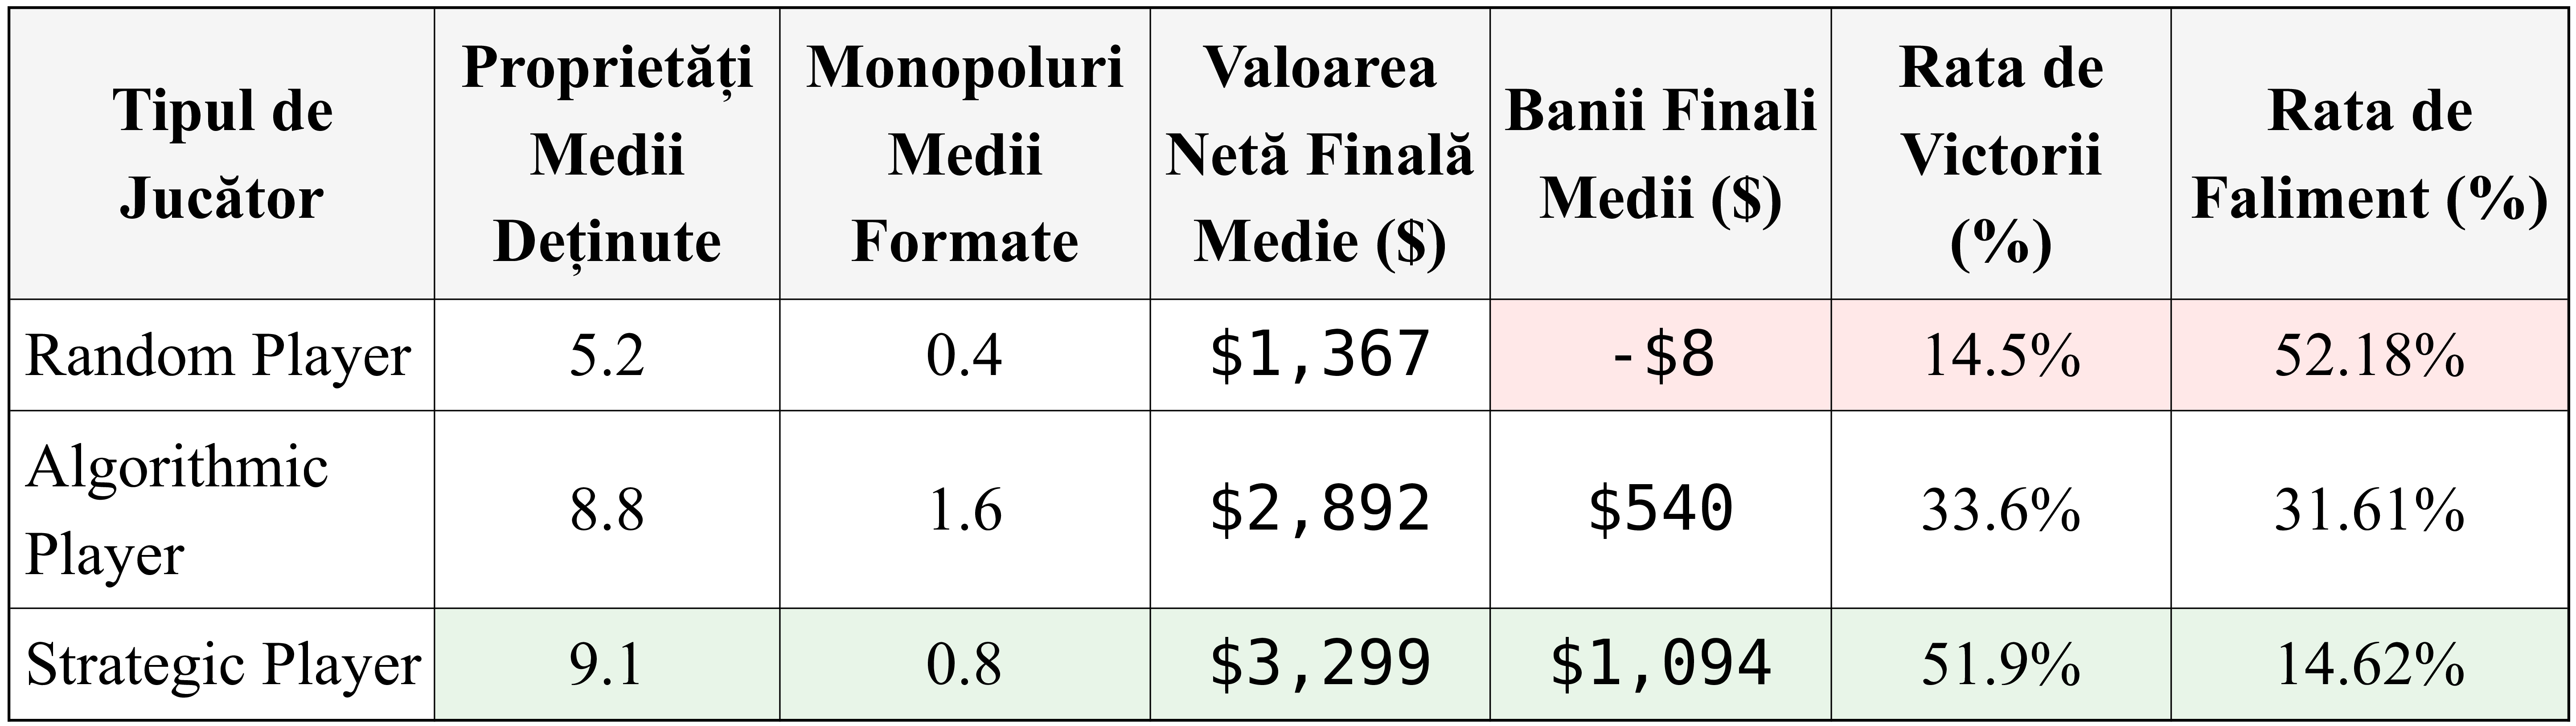
\includegraphics[width=16cm]{images/tournament_results_table.png}
    \caption{Rezultatele turneului agenților algoritmici}
    \label{fig:tournament-results-algorithmic}
\end{figure}

Suma negativă a jucătorului aleator nu este o greșeală, ci reflectă că adesea el este motivul încetării jocului, rămânând falimentar în foarte multe cazuri. Diferența dintre cei doi jucători algoritmici este una vizibilă, cel strategic preferând să aibă o rezervă cât mai mare de cash, ce îi asigură fluiditate și stabilitate.

\begin{figure}[H]
    \centering
    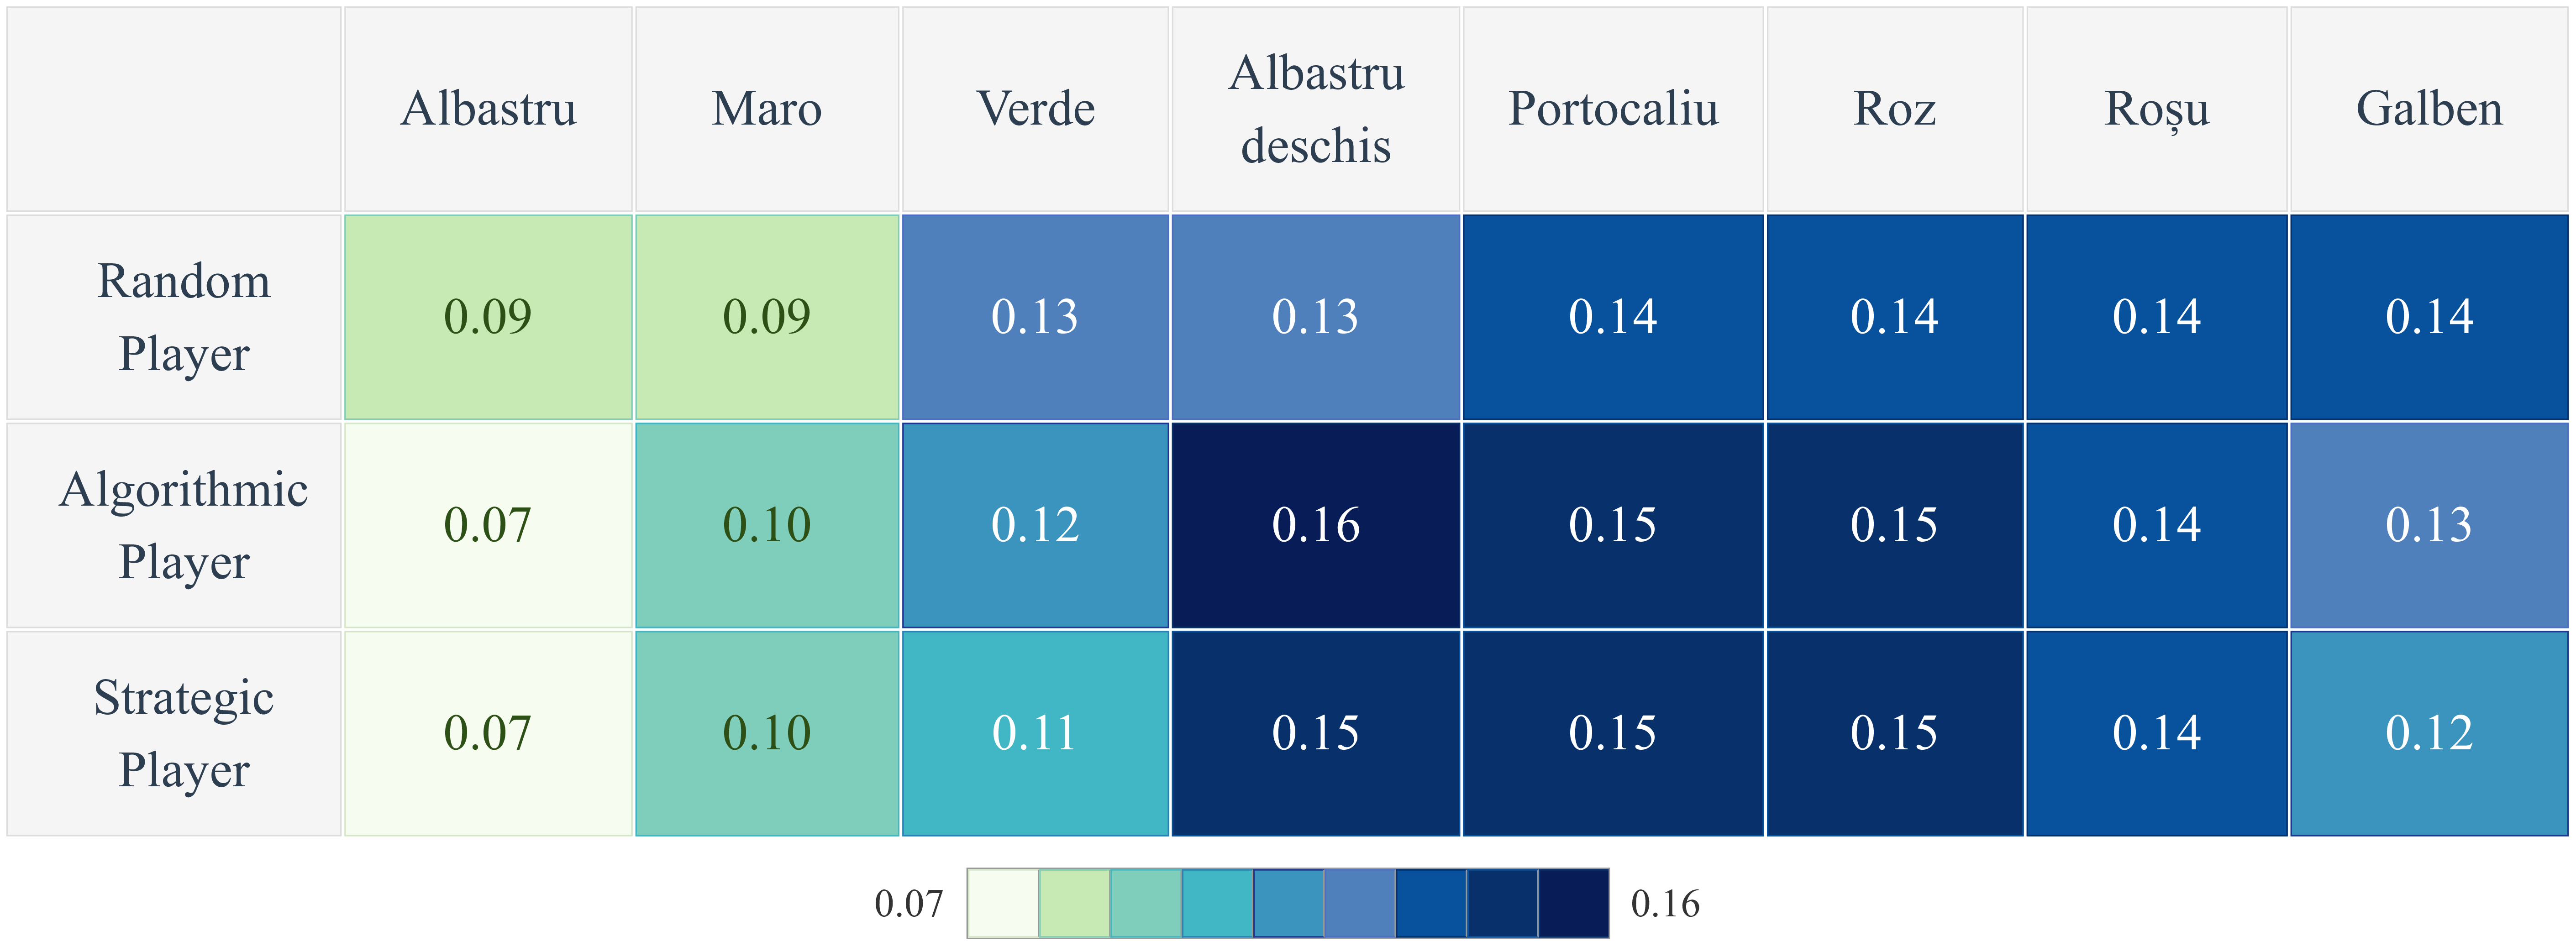
\includegraphics[width=16cm]{images/algorithmic_tournament_property_preferences.png}
    \caption{Preferințele achiziționării grupelor de culoare din turneul agenților algoritmici}
    \label{fig:tournament-results-algorithmic-property-group-preferences}
\end{figure}

În figura \ref{fig:tournament-results-algorithmic-property-group-preferences} se poate observa lipsa unei strategii definitorii în cazul agentului aleator, acesta cumpărând orice proprietate, reflectând distribuția aruncării zarurilor, frecvența fiind ridicată în jurul grupurilor de culoare vizitate regulat de jucători. Cei doi agenți algoritmici, în schimb, preferă să achiziționeze aceste proprietăți, specific grupurile de culoare albastru deschis, portocalii și roz, având o bună frecventare, dar și o bună marjă de profit.

În cazul meciurilor duel, agentul aleator a reușit să câștige în 32\% din instanțe versus agentul algoritmic și în 12\% din instanțe în fața celui strategic. Aceste numere arată, că deși deciziile sale sunt pur stocastice, acesta reușește totuși să găsească o strategie optimă. Totodată aceste numere ne indică un adevăr enunțat anterior, că o strategie universal valabilă este greu de modelat în cazul unui algoritm generalist.

Agentul strategic reușește să câștige în 67\% din instanțe față de cel algoritmic, fapt ce demonstrează că acesta este o îmbunătățire considerabilă. Diferența de 20\% în fața agentului aleator indică că strategia aleasă de agentul strategic reușește să acopere mai multe cazuri și indică o mai bună cunoaștere a mediului și a folosirii informației din acesta.

\begin{figure}[H]
    \centering
    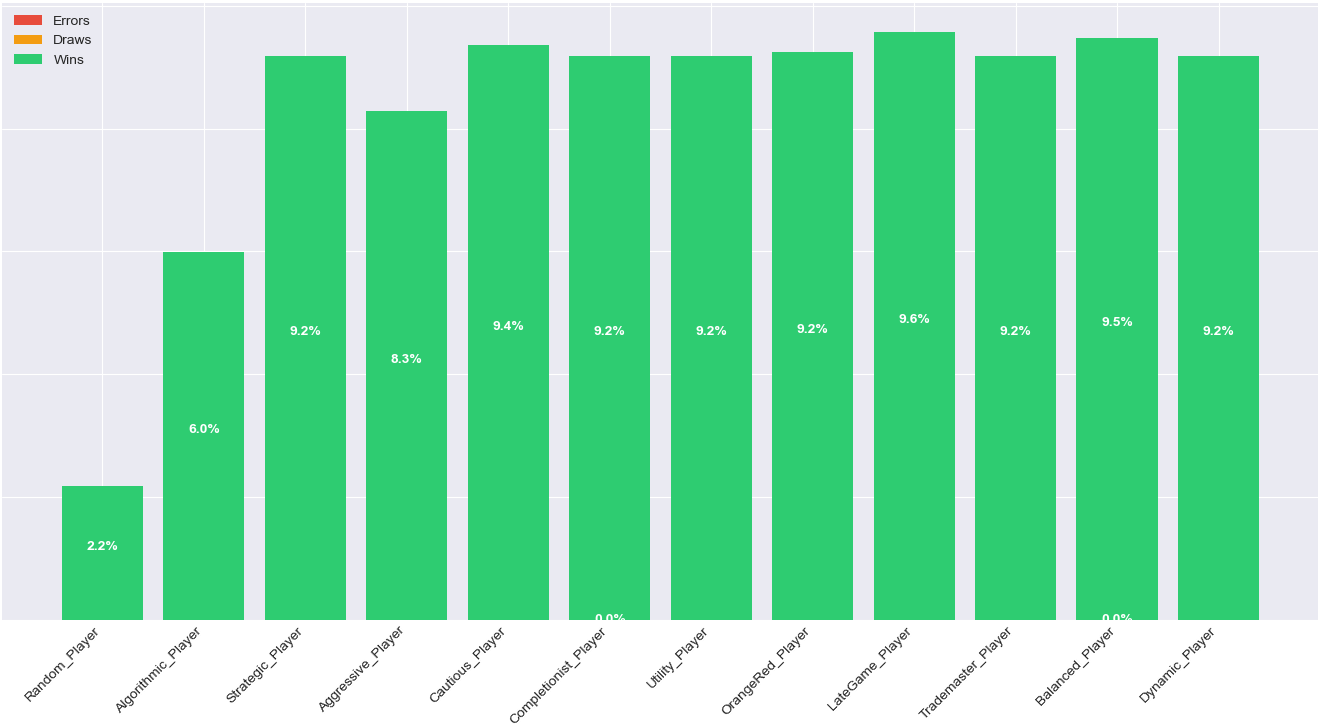
\includegraphics[width=16cm]{images/all_algorithmic agents tournament_win_rates.png}
    \caption{Rezultatele turneului round-robin pentru toți agenții algoritmici}
    \label{fig:all_algorithmic_tournament}
\end{figure}

Figura \ref{fig:all_algorithmic_tournament} prezintă rata de câștig pentru fiecare tip de agent descris până acum, într-un turneu round-robin cu 660.000 de jocuri (10.000 pentru fiecare pereche), 1.000 de runde maxime pentru fiecare joc. Așa cum se poate observa, deși are mișcări aleatoare, primul agent reușește să adune 2,2\% rată de câștig ceea ce marchează că imprevizibilitatea lui este greu de estimat de orice implementare.

La polul opus, se poate deduce că agentul strategic, cu parametrizare standard, este un jucător redutabil, având rata de câștig de 9,2\%, chiar media agenților strategici. Configurația LateGame (proiectare viitoare) este cea care reușește să se remarce cel mai bine cu o rată de câștig de 9,6\%. Atuurile acestuia sunt păstrarea unei rezerve minime de cash de cel puțin 250₩, o diferență de 100₩ față de configurația standard, și o adaptabilitate dinamică în funcție de etapele jocului, care actualizează parametrizarea agentului.

Se poate observa că media agenților strategici este 9,25\%, fiind relativ mare față de o medie a unui turneu cu agenți ce ar fi generat o rată de câștig dintr-o distribuție uniformă, 8,33\% ($100\% / 12$ (agenți)), demonstrând astfel capacitatea de adaptare și acționare într-un mediu dinamic al agenților.

\newpage
\section{Agentul uman}
În vederea interacțiunii și testării agenților, s-a realizat o interfață grafică, considerată a fi agentul uman. Aceasta are aceleași metode puse la dispoziție, iar deciziile sunt efectuate de un jucător uman.

Arhitectura agentului este una de tipul RESTful, folosind un server pe partea de backend si o interfață web pe partea de frontend. Printre tehnologiile folosite pentru realizarea interfeței grafice se enumeră: React \cite{react_dev}, Javascript \cite{mdn_javascript}, Bootstrap \cite{bootstrap}, FastAPI \cite{fastapi}, Python \cite{python_org}.

Serverul este notificat de către GameManager când un eveniment a avut loc, prin metodele legate de evenimente si păstrează cererea într-o coadă de priorități blocantă. Atunci când jocul necesită decizia jucătorului uman în privința oricărei acțiuni, se verifică existența acestei decizii în coada blocantă. În cazul în care aceasta nu există, metoda notifică interfața web despre nevoie de decizie, iar aceasta își actualizează aspectul și asteaptă pentru ca jucătorul să întreprindă o acțiune. În urma răspunsului primit de la jucator, interfața partajează acțiunea serverului, care returnează maparea la tipul cerut de metodă și încheie acțiunea curentă.

\begin{figure}[H]
    \centering
    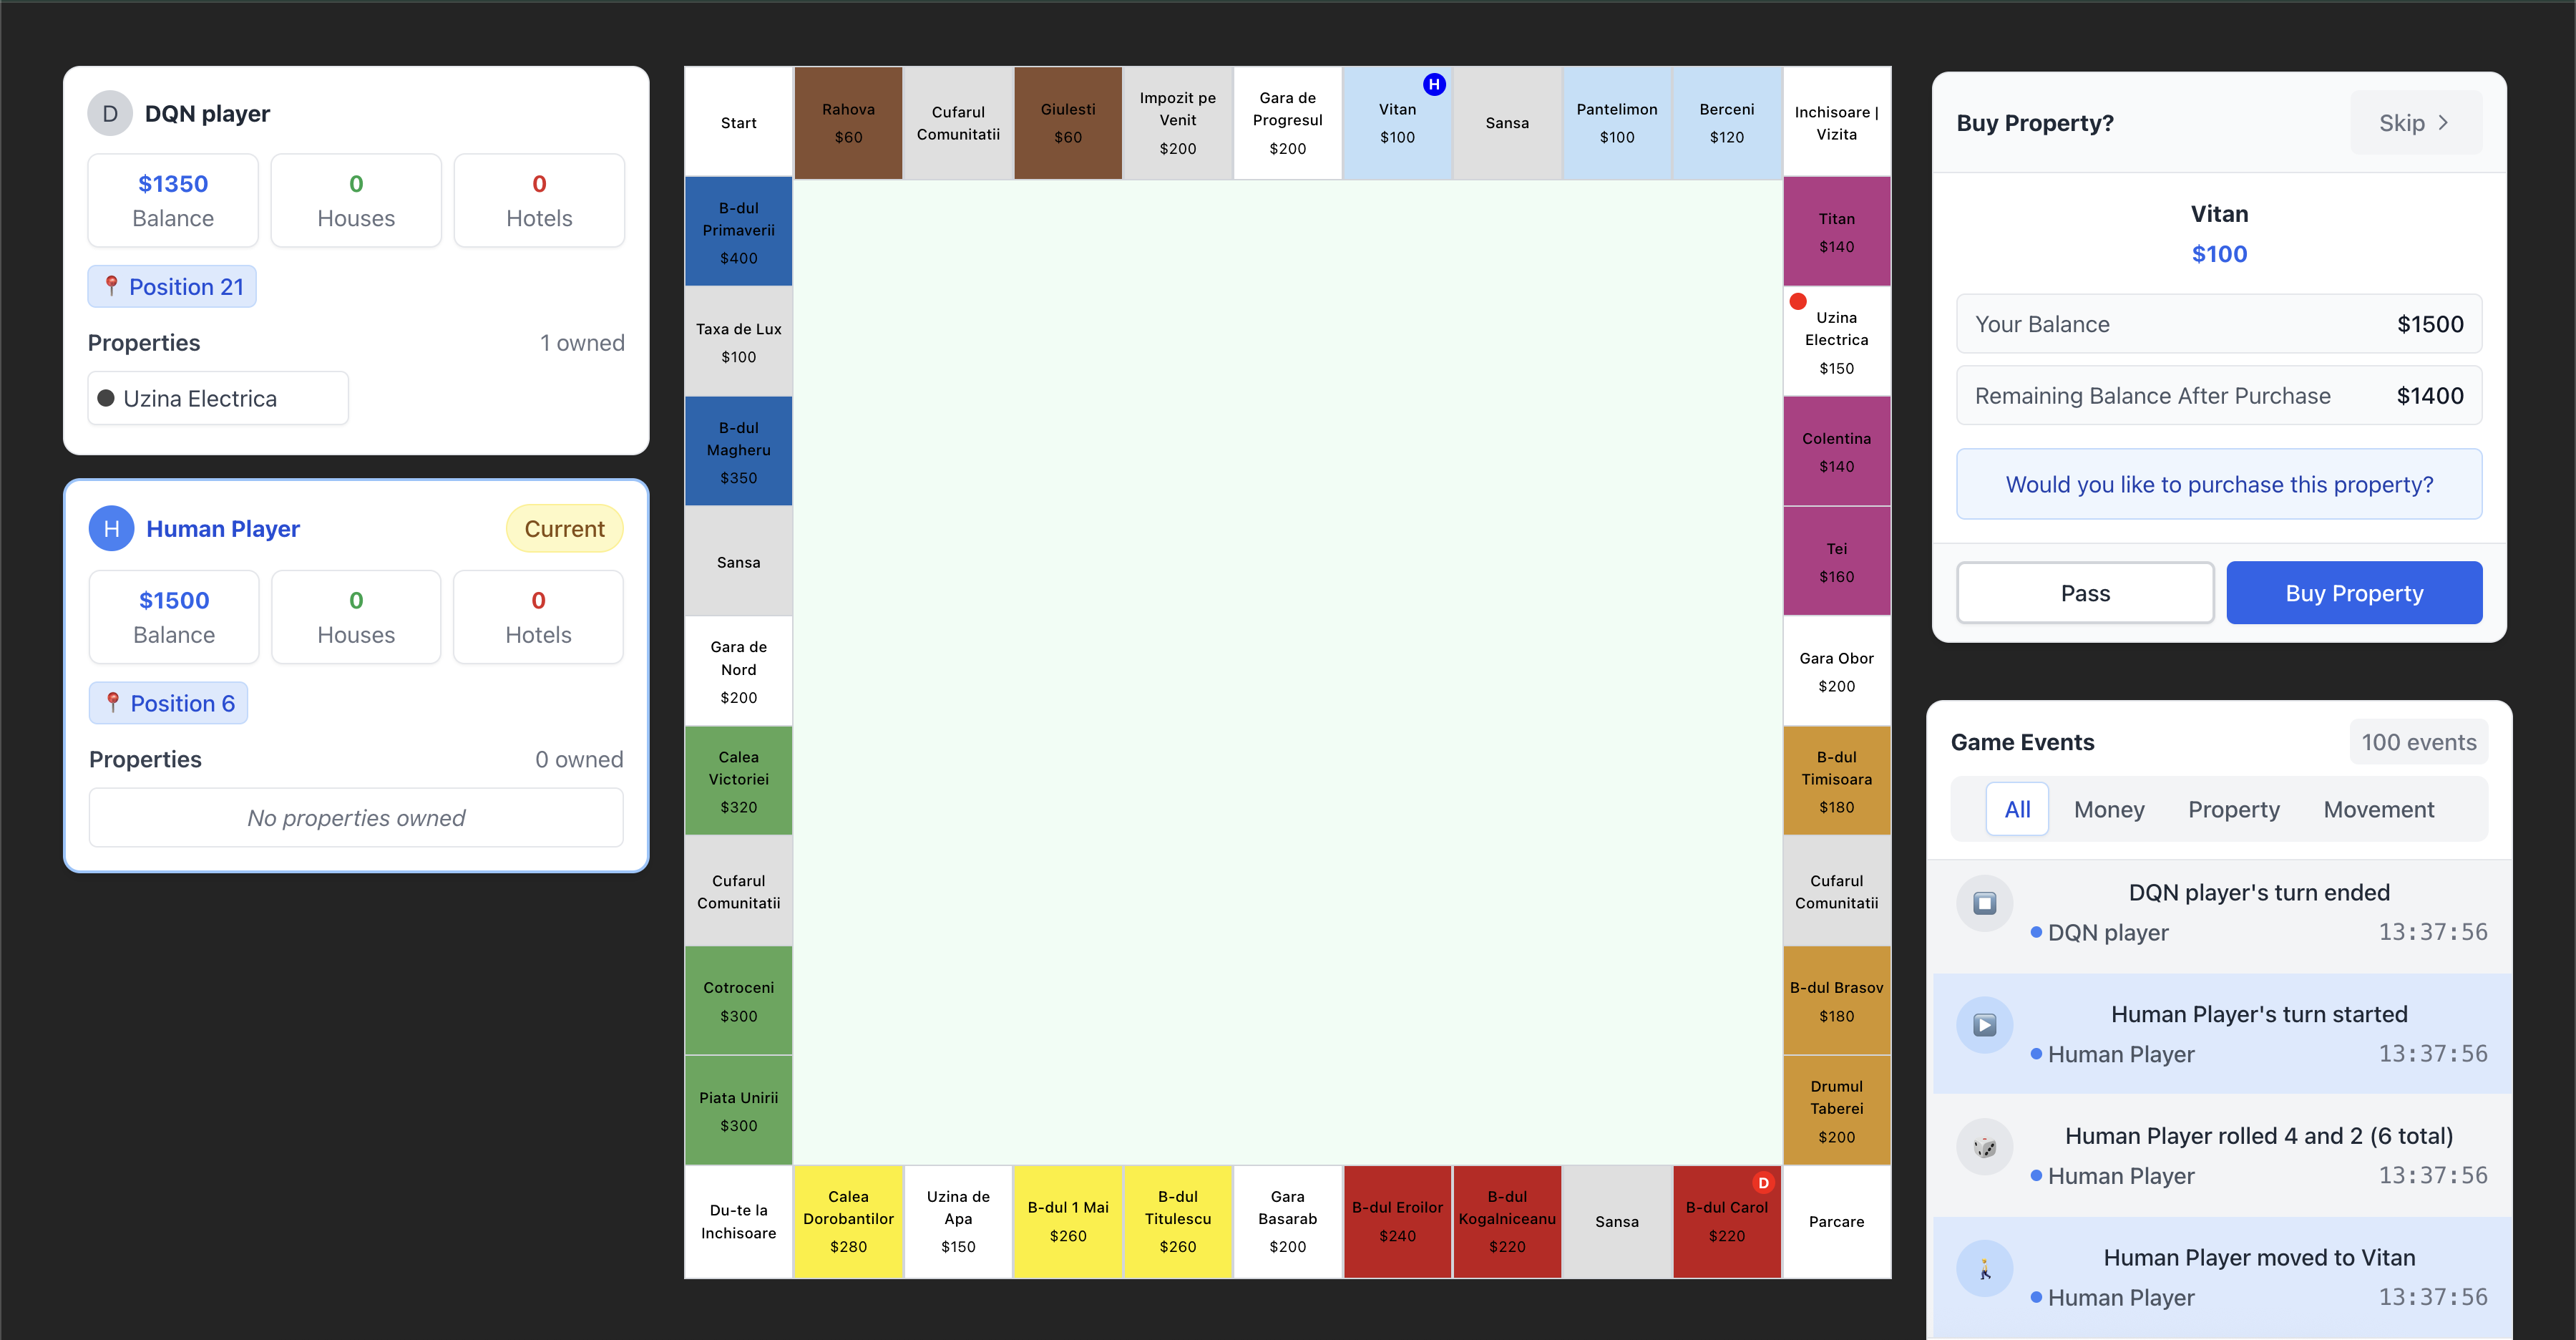
\includegraphics[width=16cm]{images/screenshot_GUI.png}
    \caption{Captură de ecran al interfeței grafice al jucătorului uman}
    \label{fig:screenshot-human-player-gui}
\end{figure}